\documentclass{article}

% if you need to pass options to natbib, use, e.g.:
%     \PassOptionsToPackage{numbers, compress}{natbib}
% before loading neurips_2020

% ready for submission
%\usepackage{neurips_2020}

% to compile a preprint version, e.g., for submission to arXiv, add add the
% [preprint] option:
%     \usepackage[preprint]{neurips_2020}

% to compile a camera-ready version, add the [final] option, e.g.:
%     \usepackage[final]{neurips_2020}

% to avoid loading the natbib package, add option nonatbib:
%\usepackage[nonatbib]{neurips_2020}

% ICML style file for CL Workshop 
\usepackage[accepted]{icml2020}
\icmltitlerunning{Supermasks in Superposition}


\usepackage[utf8]{inputenc} % allow utf-8 input
\usepackage[T1]{fontenc}    % use 8-bit T1 fonts
\usepackage{hyperref}       % hyperlinks
\usepackage{url}            % simple URL typesetting
\usepackage{booktabs}       % professional-quality tables
\usepackage{amsfonts}       % blackboard math symbols
\usepackage{nicefrac}       % compact symbols for 1/2, etc.
\usepackage{microtype}      % microtypography
\usepackage{booktabs}
\usepackage{multirow}
\usepackage[normalem]{ulem}
\usepackage{adjustbox}
\usepackage{xspace}
\usepackage{pifont}
\newcommand{\cmark}{\ding{51}}%
\newcommand{\xmark}{\ding{55}}%

%%%% ADDED IMPORTS
\usepackage{amsthm}
\usepackage{amsmath} % provides many mathematical environments & tools
\usepackage{dsfont}
%\usepackage{physics}
% \numberwithin{equation}{section}
% \usepackage{amssymb}
% \usepackage{mathtools}
% \usepackage{bbm}
% %\usepackage[colorlinks = true, urlcolor  = blue]{hyperref}
\usepackage{graphicx}
\usepackage{caption}
\usepackage{subcaption}
%\usepackage[ruled]{algorithm2e}
% \usepackage{float}
% \usepackage{titling}
% \usepackage[super]{nth}
% \usepackage{nicefrac}
% \usepackage{mathtools}
% \usepackage{cancel}
\usepackage{xcolor}
\usepackage{wrapfig}
\usepackage{tikz}
%\usepackage{algorithm}
%\usepackage{algorithmic}
%\usepackage{algpseudocode}
%\usepackage{algorithmicx,algpseudocode}
%\usepackage{algorithm}
%\usepackage[noend]{algpseudocode}
\usetikzlibrary{arrows,positioning,shapes,calc}
\tikzset{
  treenode/.style = {shape=rectangle, rounded corners,
                     draw, align=center, fill = blue!15!white}, 
  treenode2/.style = {shape=rectangle, rounded corners,
                     draw, align=center, fill = red!15!white}, 
  root/.style     = {rectangle, font=\scriptsize\bf, draw, align=center, fill=red!15!white},
  env/.style      = {treenode, font=\scriptsize\bf},
  env2/.style     = {treenode, draw=black,font=\scriptsize\bf ,fill=blue!15!white, very thick},
  env3/.style     = {treenode, font=\scriptsize\bf ,fill=green!15!white, very thick},
  newenv/.style     = {draw=none, font=\scriptsize\bf, align=center},
  whiteenv/.style     = {draw=none, font=\scriptsize, align=center},
  level2/.style     ={newenv, level distance=10cm, sibling distance=0.5em},
}

\DeclareMathOperator*{\argmax}{arg\,max}
\DeclareMathOperator*{\argmin}{arg\,min}
\DeclareMathOperator*{\hadamard}{\odot}
\DeclareMathOperator*{\diag}{diag}

% JBY: I switched the below
% Old style: math mode, tt
%\newcommand{\ac}{\ensuremath{\texttt{SupSup}}}
% New, recommended style: just text. It's just a name after all.
\newcommand{\ac}{SupSup\xspace}

\graphicspath{{../figs/}}





%%%%%%%%%%%%%%%%%%%%%%
% DC Commenting highlights
%%%%%%%%%%%%%%%%%%%%%%

% % Commenting highlights
\newif\ifcomments

%Uncomment one of the two lines below to turn todos on/off
\commentsfalse
%\commentstrue

\ifcomments
\newcommand{\comments}[1]{#1}
\else
\newcommand{\comments}[1]{}
\fi
% % Commenting highlights

%\providecommand{\ali}[1]{{\protect\color{red}{\bf [ali: #1]}}}
%\providecommand{\vivekr}[1]{{\protect\color{purple}{\bf [vivek: #1]}}}
%\providecommand{\mitch}[1]{{\protect\color{blue}{[mitch: #1]}}}
%\providecommand{\rosanne}[1]{{\protect\color{magenta}{[rosanne: #1]}}}
\newcommand{\ali}[1]{\comments{\textcolor{red}{[ali: #1]}}}
\newcommand{\vivekr}[1]{\comments{\textcolor{purple}{[vivek: #1]}}}
\newcommand{\mitch}[1]{\comments{\textcolor{blue}{[mitch: #1]}}}
\newcommand{\rosanne}[1]{\comments{\textcolor{magenta}{[rosanne: #1]}}}
\newcommand{\jby}[1]{\comments{\textcolor{orange}{[JBY: #1]}}}

\newcommand{\later}[1]{\comments{\textcolor{green}{[Later: #1]}}}
\definecolor{muchlater}{rgb}{0.7,1,.7}
\newcommand{\muchlater}[1]{\comments{\textcolor{muchlater}{[Much Later: #1]}}}
\newcommand{\maybe}[1]{\comments{\textcolor{lightgray}{[Maybe: #1]}}}
\newcommand{\removed}[1]{\comments{\textcolor{lightgray}{#1}}}
\newcommand{\verify}[1]{\comments{\textcolor{gray}{[verify] #1}}}
\newcommand{\replace}[1]{\comments{\textcolor{gray}{[replace-with-actual] #1}}}



\newcommand{\casename}[1]{\ensuremath{\mathsf{#1}}\xspace}

% Refs and labels
\newcommand{\figlabel}[1]{\label{fig:#1}}
\newcommand{\figref}[1]{Figure~\ref{fig:#1}}
\newcommand{\figsref}[2]{Figures~\ref{fig:#1} \& \ref{fig:#2}}
\newcommand{\seclabel}[1]{\label{sec:#1}}
\newcommand{\secref}[1]{Section~\ref{sec:#1}}
\newcommand{\tablabel}[1]{\label{tab:#1}}
\newcommand{\tabref}[1]{Table~\ref{tab:#1}}
\newcommand{\eqnlabel}[1]{\label{eqn:#1}}
\newcommand{\eqnref}[1]{Equation~\ref{eqn:#1}}
\newcommand{\alglabel}[1]{\label{alg:#1}}
%\newcommand{\algref}[1]{Algorithm~\ref{alg:#1}}


%%%% END
\begin{document}

\twocolumn[
\icmltitle{Supermasks in Superposition}

% It is OKAY to include author information, even for blind
% submissions: the style file will automatically remove it for you
% unless you've provided the [accepted] option to the icml2020
% package.

% List of affiliations: The first argument should be a (short)
% identifier you will use later to specify author affiliations
% Academic affiliations should list Department, University, City, Region, Country
% Industry affiliations should list Company, City, Region, Country

% You can specify symbols, otherwise they are numbered in order.
% Ideally, you should not use this facility. Affiliations will be numbered
% in order of appearance and this is the preferred way.
\icmlsetsymbol{equal}{*}

\begin{icmlauthorlist}
\icmlauthor{Mitchell Wortsman}{equal,uw}
\icmlauthor{Vivek Ramanujan}{equal,ai}
\icmlauthor{Rosanne Liu}{ml}
\icmlauthor{Aniruddha Kembhavi}{uw,ai}
\icmlauthor{Mohammad Rastegari}{uw}
\icmlauthor{Jason Yosinski}{ml}
\icmlauthor{Ali Farhadi}{uw}
\end{icmlauthorlist}
    % Uiversity of Washington \\
    % \And
    %   Vivek Ramanujan$^*$ \\
    % Allen Institute for AI \\
    %     \And
    %   Rosanne Liu \\
    % ML Collective \\
    %     \And
    %   Aniruddha Kembhavi$^\dagger$ \\
    % Allen Institute for AI \\
    %     \And
    %   Mohammad Rastegari \\
    % University of Washington \\
    %         \And
    %   Jason Yosinski \\
    % ML Collective \\
    %     \And
    %   Ali Farhadi \\
    % University of Washington \\

\icmlaffiliation{uw}{University of Washington}
\icmlaffiliation{ai}{Allen Institute for AI}
\icmlaffiliation{ml}{ML Collective}

\icmlcorrespondingauthor{Mitchell Wortsman}{mitchnw@cs.washington.edu}
%\icmlcorrespondingauthor{Eee Pppp}{ep@eden.co.uk}

% You may provide any keywords that you
% find helpful for describing your paper; these are used to populate
% the "keywords" metadata in the PDF but will not be shown in the document
\icmlkeywords{Machine Learning, ICML}

\vskip 0.3in
]

\printAffiliationsAndNotice{\icmlEqualContribution} % otherwise use the standard text.

% The \author macro works with any number of authors. There are two commands
% used to separate the names and addresses of multiple authors: \And and \AND.
%
% Using \And between authors leaves it to LaTeX to determine where to break the
% lines. Using \AND forces a line break at that point. So, if LaTeX puts 3 of 4
% authors names on the first line, and the last on the second line, try using
% \AND instead of \And before the third author name.



% theorem styles
\theoremstyle{plain}
\newtheorem{theorem}{Theorem}[section]
\newtheorem{corollary}{Corollary}[theorem]
\newtheorem{lemma}[theorem]{Lemma}
\newtheorem{proposition}[theorem]{Proposition}

\theoremstyle{definition}
\newtheorem{definition}[theorem]{Definition}
\newtheorem{remark}[theorem]{Remark}

% brackets
\newcommand{\round}[1]{\left( #1 \right)}
\newcommand{\curly}[1]{\left\lbrace #1 \right\rbrace}
\newcommand{\squarebrack}[1]{\left\lbrack #1 \right\rbrack}

% sums
\newcommand{\sumi}[2]{\sum\limits_{i=#1}^{#2}}
\newcommand{\sumj}[2]{\sum\limits_{j=#1}^{#2}}
\newcommand{\sumk}[2]{\sum\limits_{k=#1}^{#2}}
\newcommand{\sump}[2]{\sum\limits_{p=#1}^{#2}}
\newcommand{\suml}[2]{\sum\limits_{l=#1}^{#2}}
\newcommand{\sumn}[2]{\sum\limits_{n=#1}^{#2}}
\newcommand{\summ}[2]{\sum\limits_{m=#1}^{#2}}
\newcommand{\sumt}[2]{\sum\limits_{t=#1}^{#2}}

\newcommand{\Sum}{\sum_{i = 1}^{n}}
\newcommand{\Sumi}[1]{\sum\limits_{i = 1}^{#1}}
\newcommand{\Sumt}[1]{\sum\limits_{t = 1}^{#1}}

% norms
\newcommand{\abs}[1]{\left\lvert #1 \right\rvert}
\newcommand{\norm}[2]{\left\lVert#2\right\rVert_{#1}}
\newcommand{\esqnorm}[1]{\left\lVert#1\right\rVert_2^2}
\newcommand{\enorm}[1]{\left\lVert#1\right\rVert_2}
\newcommand{\infnorm}[1]{\left\lVert#1\right\rVert_\infty}
\newcommand{\opnorm}[1]{\left\lVert#1\right\rVert_\text{op}}
\newcommand{\normF}[1]{\left\lVert#1\right\rVert_{\text{F}}}
\newcommand{\inner}[1]{\left\langle#1\right\rangle}
\newcommand{\ceil}[1]{\left\lceil#1\right\rceil}
\newcommand{\floor}[1]{\left\lfloor#1\right\rfloor}

% bold numbers
\newcommand{\zero}{\mathbf{0}}
\newcommand{\one}{\mathbf{1}}

% bold small english vectors
\newcommand{\avec}{\mathbf{a}}
\newcommand{\bvec}{\mathbf{b}}
\newcommand{\cvec}{\mathbf{c}}
\newcommand{\dvec}{\mathbf{d}}
\newcommand{\e}{\mathbf{e}}
\newcommand{\f}{\mathbf{f}}
\newcommand{\g}{\mathbf{g}}
\newcommand{\h}{\mathbf{h}}
\newcommand{\ivec}{\mathbf{i}}
\newcommand{\jvec}{\mathbf{j}}
\newcommand{\kvec}{\mathbf{k}}
\newcommand{\lvec}{\mathbf{l}}
\newcommand{\m}{\mathbf{m}}
\newcommand{\n}{\mathbf{n}}
\newcommand{\ovec}{\mathbf{o}}
\newcommand{\p}{\mathbf{p}}
\newcommand{\q}{\mathbf{q}}
\newcommand{\rvec}{\mathbf{r}}
\newcommand{\s}{\mathbf{s}}
\newcommand{\tvec}{\mathbf{t}}
\newcommand{\uvec}{\mathbf{u}}
\newcommand{\vvec}{\mathbf{v}}
\newcommand{\w}{\mathbf{w}}
\newcommand{\x}{\mathbf{x}}
\newcommand{\y}{\mathbf{y}}
\newcommand{\z}{\mathbf{z}}

% bold capital english matrices
\newcommand{\A}{\mathbf{A}}
\newcommand{\B}{\mathbf{B}}
\newcommand{\C}{\mathbf{C}}
\newcommand{\D}{\mathbf{D}}
\newcommand{\Emat}{\mathbf{E}}
\newcommand{\F}{\mathbf{F}}
\newcommand{\G}{\mathbf{G}}
\newcommand{\Hmat}{\mathbf{H}}
\newcommand{\I}{\mathbf{I}}
\newcommand{\J}{\mathbf{J}}
\newcommand{\K}{\mathbf{K}}
\newcommand{\Lmat}{\mathbf{L}}
\newcommand{\M}{\mathbf{M}}
\newcommand{\N}{\mathbf{N}}
\newcommand{\Omat}{\mathbf{O}}
\newcommand{\Pmat}{\mathbf{P}}
\newcommand{\Q}{\mathbf{Q}}
\newcommand{\Rmat}{\mathbf{R}}
\newcommand{\Smat}{\mathbf{S}}
\newcommand{\T}{\mathbf{T}}
\newcommand{\U}{\mathbf{U}}
\newcommand{\V}{\mathbf{V}}
\newcommand{\W}{\mathbf{W}}
\newcommand{\X}{\mathbf{X}}
\newcommand{\Y}{\mathbf{Y}}
\newcommand{\Z}{\mathbf{Z}}

% bold capital greek matrices
\newcommand{\SIGMA}{\mathbf{\Sigma}}
\newcommand{\LAMBDA}{\mathbf{\Lambda}}

% capital mathcal
\newcommand{\Acal}{\mathcal{A}}
\newcommand{\Bcal}{\mathcal{B}}
\newcommand{\Ccal}{\mathcal{C}}
\newcommand{\Dcal}{\mathcal{D}}
\newcommand{\Ecal}{\mathcal{E}}
\newcommand{\Fcal}{\mathcal{F}}
\newcommand{\Gcal}{\mathcal{G}}
\newcommand{\Hcal}{\mathcal{H}}
\newcommand{\Ical}{\mathcal{I}}
\newcommand{\Jcal}{\mathcal{J}}
\newcommand{\Kcal}{\mathcal{K}}
\newcommand{\Lcal}{\mathcal{L}}
\newcommand{\Mcal}{\mathcal{M}}
\newcommand{\Ncal}{\mathcal{N}}
\newcommand{\Ocal}{\mathcal{O}}
\newcommand{\Pcal}{\mathcal{P}}
\newcommand{\Qcal}{\mathcal{Q}}
\newcommand{\Rcal}{\mathcal{R}}
\newcommand{\Scal}{\mathcal{S}}
\newcommand{\Tcal}{\mathcal{T}}
\newcommand{\Ucal}{\mathcal{U}}
\newcommand{\Vcal}{\mathcal{V}}
\newcommand{\Wcal}{\mathcal{W}}
\newcommand{\Xcal}{\mathcal{X}}
\newcommand{\Ycal}{\mathcal{Y}}
\newcommand{\Zcal}{\mathcal{Z}}

% small greek bold vectors
\newcommand{\alphavec}{\boldsymbol{\alpha}}
\newcommand{\betavec}{\boldsymbol{\beta}}
\newcommand{\gammavec}{\boldsymbol{\gamma}}
\newcommand{\deltavec}{\boldsymbol{\delta}}
\newcommand{\epsvec}{\boldsymbol{\epsilon}}
\newcommand{\etavec}{\boldsymbol{\eta}}
\newcommand{\nuvec}{\boldsymbol{\nu}}
\newcommand{\tauvec}{\boldsymbol{\tau}}
\newcommand{\rhovec}{\boldsymbol{\rho}}
\newcommand{\lmbda}{\boldsymbol{\lambda}}
\newcommand{\muvec}{\boldsymbol{\mu}}
\newcommand{\thetavec}{\boldsymbol{\theta}}

% complexity notations
\newcommand{\BigO}[1]{\mathcal{O}\round{#1}}
\newcommand{\BigOmega}[1]{\Omega\round{#1}}

% Set notations
\newcommand{\R}{\mathbb{R}}
\newcommand{\Rd}[1]{\mathbb{R}^{#1}}
\newcommand{\Natural}{\mathbb{N}}
\newcommand{\Complex}{\mathbb{C}}
\newcommand{\Integer}{\mathbb{Z}}
\newcommand{\Rational}{\mathbb{Q}}

% Probability
\newcommand{\E}[1]{\mathbb{E}\squarebrack{#1}}
\newcommand{\Exp}[2]{\mathbb{E}_{#1}\squarebrack{#2}}
\newcommand{\Prob}[1]{\mathds{P}\squarebrack{#1}}
\newcommand{\Probability}[2]{P_{#1}\curly{#2}}
\newcommand{\Var}[1]{\mathrm{Var}\squarebrack{#1}}
\newcommand{\Cov}[1]{\mathrm{Cov}\squarebrack{#1}}
\newcommand{\PR}[1]{\mathds{P}\round{#1}}

% math shortcuts
\newcommand{\inv}[1]{\frac{1}{#1}}
\newcommand{\indicator}[2]{\mathbbm{1}_{#1}\squarebrack{#2}}
\newcommand{\Tr}[1]{\text{Tr}\squarebrack{#1}}

% others
\newcommand{\BOX}[1]{\fbox{\parbox{\linewidth}{\centering#1}}}
\newcommand{\textequal}[1]{\stackrel{#1}{=}}
\newcommand{\textleq}[1]{\stackrel{#1}{\leq}}
\newcommand{\textgeq}[1]{\stackrel{#1}{\geq}}
\newcommand{\defeq}{\vcentcolon=}

% calculus
\newcommand{\dd}[2]{\frac{d #1}{d #2}}
\newcommand{\ddn}[3]{\frac{d^{#1} #2}{d #3^{#1}}}
\newcommand{\dodo}[2]{\frac{\partial #1}{\partial #2}}
\newcommand{\dodon}[3]{\frac{\partial^{#1} #2}{\partial {#3}^{#1}}}


%\maketitle




\begin{abstract}
    We present Supermasks in Superposition (SupSup), a model capable of sequentially learning thousands of tasks without catastrophic forgetting. Our approach uses a randomly initialized, fixed base network and for each task finds a subnetwork (supermask) that achieves good performance. If task identity is given at test time, the correct subnetwork can be retrieved with minimal compute. If not provided, SupSup can infer the task using gradient-based optimization to find a linear superposition of learned supermasks which minimizes the output entropy. In practice we find that a single gradient step can be sufficient to identify the correct mask, even among 2500 tasks. A more complete version of this paper is available at  \url{https://arxiv.org/abs/2006.14769}.\removed{We also showcase two promising extensions. First, SupSup models can be trained entirely without task identity information, as they may detect when they are uncertain about new data and allocate an additional supermask for the new training distribution. Finally the entire, growing set of supermasks can be stored in a constant-sized reservoir by implicitly storing them as attractors in a fixed-sized Hopfield network.}
\end{abstract}



\section{Introduction}

Learning many different tasks sequentially without \emph{catastrophic forgetting} \cite{mccloskey1989catastrophic,french1999catastrophic, goodfellow2013empirical} remains a notable challenge for neural networks. \removed{\cite{thrun1998lifelong, zhao1996incremental, kirkpatrick2017overcoming}.}
In this paper, we begin with the observation that catastrophic forgetting cannot occur if the weights of the network remain fixed and random. We leverage this to develop a flexible model capable of learning thousands of tasks: \textit{Supermasks in Superposition} (\ac). \ac, diagrammed in \figref{teaser}, is driven by two core ideas: \textbf{a)} the expressive power of untrained, randomly weighted subnetworks \cite{zhou2019deconstructing, ramanujan2019s}, and \textbf{b)} inference of task-identity with gradient-based optimization.

\textbf{a) The expressive power of subnetworks}
\removed{Neural networks may be overlaid with a binary mask that selectively keeps or removes each connection, producing a subnetwork.
The number of possible subnetworks is combinatorial in the number of parameters.} Researchers have observed that \removed{the number of combinations is large enough 
that }even within randomly weighted neural networks, there exist subnetworks which achieve good performance on complex tasks. \citet{zhou2019deconstructing} and \citet{ramanujan2019s} present two algorithms for finding these subnetworks by training \emph{supermasks}. \removed{while keeping the weights of the underlying network fixed and random.}
SupSup solves sequential tasks by finding for each task a supermask atop a shared, untrained network.


\textbf{b) Inference of task-identity as an optimization problem}
When task identity is unknown, $\text{\ac}$ can infer task identity to select the correct supermask.
\removed{Given data from unknown task, the correct supermask originally trained for the same task should exhibit a confident (\textit{i.e.} low entropy) output distribution \cite{hendrycks2016baseline}, so we} We frame inference of task-identity as an optimization problem: finding the convex combination of learned supermasks which minimizes the entropy of the output distribution.

We propose a new taxonomy of continual learning scenarios (\secref{cl}), and develop and evaluate \ac via all scenarios: whether task ID is provided during train and test (\casename{GG}), during train but not test (\casename{GN}), or not provided at all (\casename{NNs}). 
\begin{figure}[t]
    \centering
    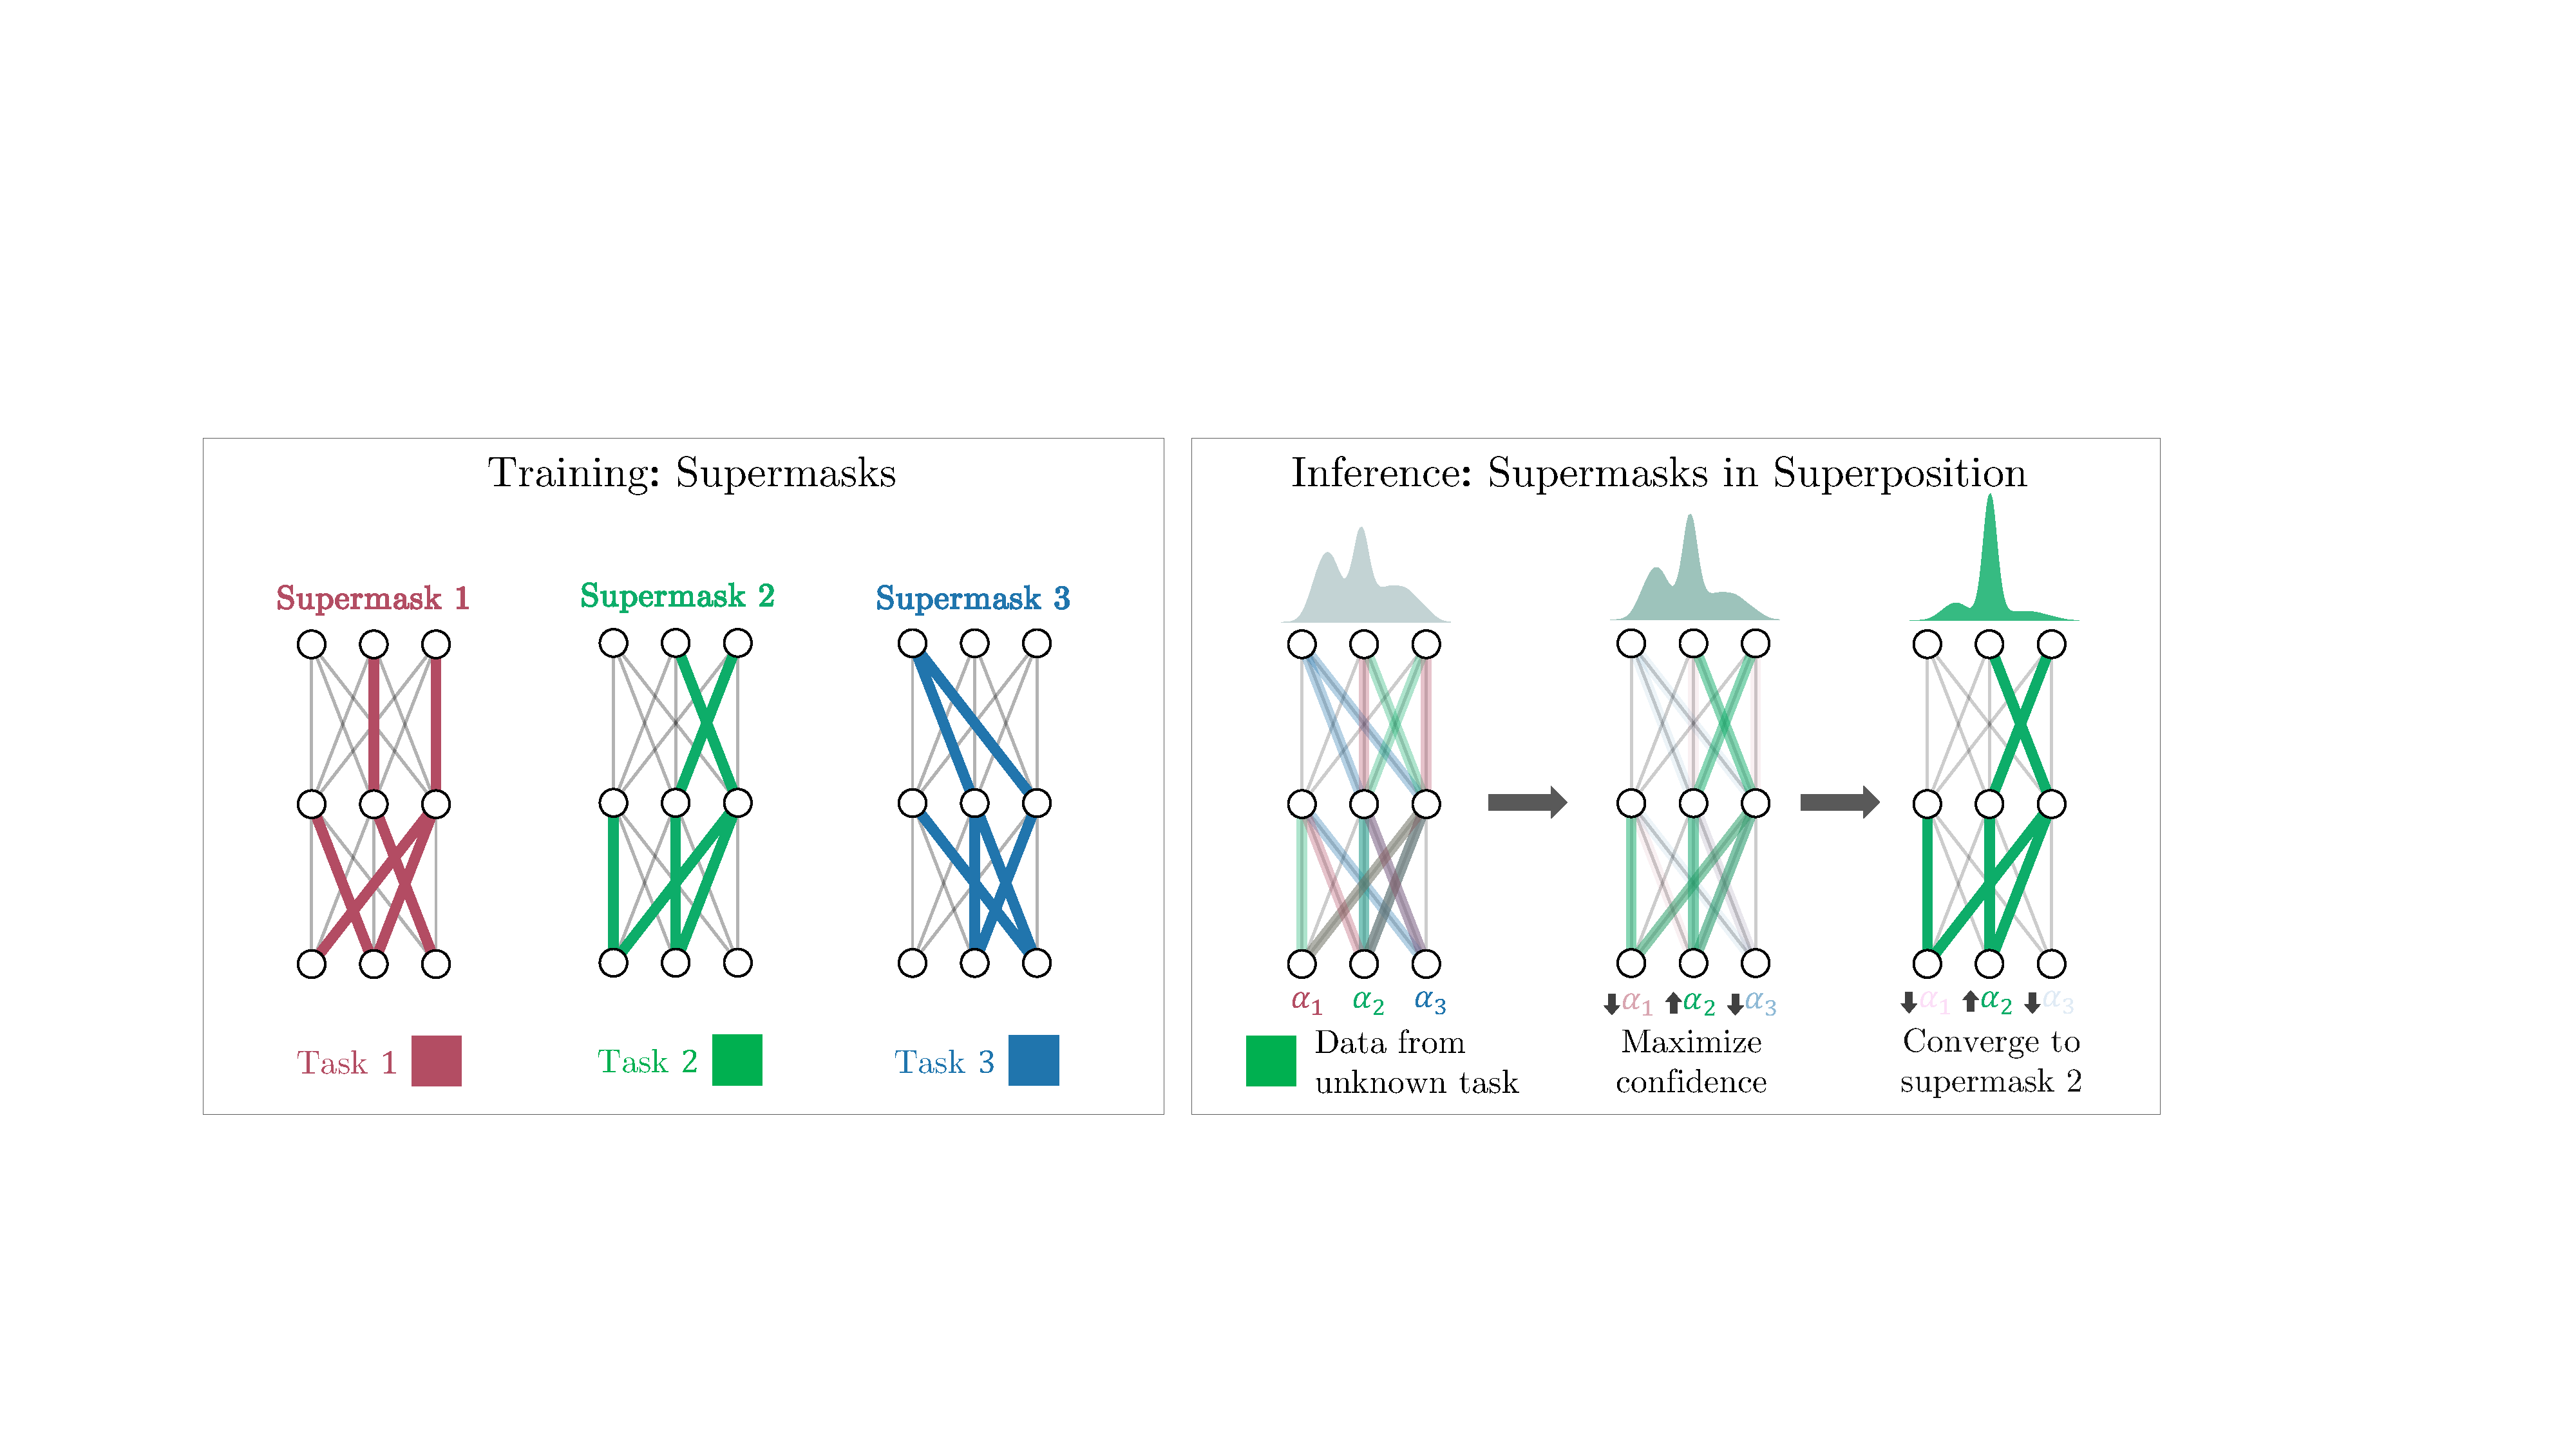
\includegraphics[width=0.5\textwidth]{figs/teaser_ppt.pdf}
    \caption{\textbf{(left)} During training \ac learns a separate supermask (subnetwork) for each task. \textbf{(right)} At inference time, \ac can infer task identity by superimposing all supermasks, each weighted by an $\alpha_i$, and using gradients to adjust $\alpha$ values to maximize confidence on unknown data.}
    \vspace*{-1em}
    \figlabel{teaser}
\end{figure}

\vspace*{-1ex}
\section{Continual Learning Scenarios \removed{and Related Work}}
\label{sec:cl}


In continual learning, a model aims to solve a number of tasks sequentially \cite{thrun1998lifelong, zhao1996incremental} without catastrophic forgetting.
Although numerous approaches have been proposed in the context of continual learning, there lacks a convention of  scenarios in which methods are trained and evaluated~\cite{van2019three}. The key identifiers of scenarios include: \textbf{1)} whether task identity is provided during training, \textbf{2)} provided during inference, \textbf{3)} whether class labels are shared during evaluation, 
and \textbf{4)} whether the overall task space is discrete or continuous.
This results in an exhaustive set of 16 possibilities, many of which are invalid or uninteresting. For example, 
if task identity is never provided in training, providing it in inference is no longer helpful.
To that end, we highlight four applicable scenarios, each with a further breakdown of discrete vs. continuous, when applicable, as shown in~\tabref{scenarios}.
%
We decompose continual learning scenarios via a three-letter taxonomy that explicitly addresses the three most critical scenario variations. 
The first two letters specify whether task identity is given during training (\casename{G} if given, \casename{N} if not) and during inference (\casename{G} if given, \casename{N} if not).
The third letter specifies a subtle but important distinction: whether labels are shared (\casename{s}) across tasks or not (\casename{u}).
In the unshared case, the model must predict both the correct task ID and the correct class within that task. In the shared case, the model need only predict the correct, shared label across tasks, so it need not predict which task the data came from.
\removed{For example, when learning 5 permutations of MNIST in the \casename{GN} scenario (task IDs given during train but not test), a shared label \casename{GNs} scenario will evaluate the model on the correct predicted label across 10 possibilities, while in the unshared \casename{GNu} case the model must predict across 50 possibilities, a more difficult problem.}

A full expansion of possibilities entails both \casename{GGs} and \casename{GGu}, but as \casename{s} and \casename{u} describe only model \emph{evaluation}, any model capable of predicting shared labels can predict unshared equally well using the provided task ID at test time. Thus these cases are equivalent, and we designate both \casename{GG}.
Moreover,
the \casename{NNu} scenario is invalid because unseen labels signal the presence of a new task (the ``labels trick'' in \cite{zeno2018task}), making the scenario actually \casename{GNu}, and so we consider only the shared label case \casename{NNs}.

\removed{As to the discrete vs. continuous distinction, the taxonomy applies equivalently to discrete domains with integer ``Task IDs'' as to continue domains with ``Task Embedding'' or ``Task Context'' vectors. The remainder of this paper follows the majority of extant literature in focusing on the case with discrete task boundaries. (see e.g. \cite{ zeno2018task} for progress in the continuous scenario).}
\removed{Equipped with this taxonomy, }
We now review existing task-specific approaches for continual learning---methods which use different model components for each task. In Section~\ref{sec:ext-rw} we review approaches using regularization, generative models, or replay.

\begin{table*}[t]
  \caption{Overview of different Continual Learning scenarios. We suggest scenario names that provide an intuitive understanding of the variations in training, inference, and evaluation, while allowing a full coverage of the scenarios previously defined in~\citet{van2019three} and~\citet{zeno2018task}. See text for more complete description.
    \muchlater{can we cover regression, unsupervised learning, and RL too?}
}
\label{tab:scenarios}
\vspace*{-1.5ex}
\centering
\begin{adjustbox}{width=1\textwidth}
\begin{tabular}{@{}l l l l@{}}
\toprule
\multirow{2}{*}{Scenario} &
  \multirow{2}{*}{Description} &
  \multirow{2}{*}{\begin{tabular}[c]{@{}l@{}}Task space discreet\\ or continuous?\end{tabular}} &
  \multirow{2}{*}{\begin{tabular}[c]{@{}l@{}}Example methods / \\ task names used\end{tabular}} \\
 &
   &
   &
   \\ \midrule
  \casename{GG} &
  Task \textbf{G}iven during train and \textbf{G}iven during inference &
  Either &

  \begin{tabular}[c]{@{}l@{}}PNN~\cite{rusu2016progressive}, BatchE~\cite{wen2020batchensemble}, PSP~\cite{cheung2019superposition}, ``Task learning''~\cite{zeno2018task}, ``Task-IL''~\cite{van2019three} \end{tabular} \\ \midrule
    \casename{GNs} & Task \textbf{G}iven during train, \textbf{N}ot inference; \textbf{s}hared labels      & Either          & EWC~\cite{kirkpatrick2017overcoming}, SI \cite{zenke2017continual}, ``Domain learning''~\cite{zeno2018task}, ``Domain-IL''~\cite{van2019three} \\ \midrule
    \casename{GNu} & Task \textbf{G}iven during train, \textbf{N}ot inference; \textbf{u}nshared labels & Discrete only &    ``Class learning''~\cite{zeno2018task}, ``Class-IL''~\cite{van2019three}                                                              \\ \midrule
\casename{NNs} &
  Task \textbf{N}ot given during train \textbf{N}or inference; \textbf{s}hared labels &
  Either &
  BGD, ``Continuous/discrete task agnostic learning''~\cite{zeno2018task} \\ \bottomrule
\end{tabular}
\end{adjustbox}
\vspace*{-2.5ex}
\end{table*}
In Progressive Neural Networks (PNN)~\cite{rusu2016progressive}, Dynamically Expandable Networks~\cite{yoon2017lifelong} and Reinforced Continual Learning~\cite{xu2018reinforced}, the model is expanded for each new task. More efficiently, \cite{masse2018alleviating} fixes the network size and randomly assigns active nodes for given tasks. In \cite{mallya2018packnet, golkar2019continual}, weights of disjoint subnetworks are trained for each task. Instead of learning the weights of the subnetwork, \citet{mallya2018piggyback} learn a binary mask per task that is applied to a network pretrained on ImageNet. 
%
Recently, \citet{cheung2019superposition} superimpose many models into one by using different contexts for each task.\removed{The task parameters can then be effectively retrieved using the correct task context.}
Finally, BatchE~\cite{wen2020batchensemble} learns a shared weight matrix on the first task and only a rank-one elementwise scaling matrix for each subsequent task.

Our method can be characterized as task-specific as it introduces task-specific supermasks.
However, while all other methods in this category are limited to the \casename{GG} scenario, SupSup can be used to achieve compelling performance in \emph{all four scenarios}.
We compare primarily with BatchE~\cite{wen2020batchensemble} and Parameter Superposition (abbreviated PSP) \cite{cheung2019superposition} as they are recent and performative. \removed{BatchE requires very few additional parameters for each new task while achieving comparable performance to PNN and scaling to SplitImagenet. Moreover, PSP outperforms regularization based approaches like SI \cite{zenke2017continual}.}
However, both BatchE and PSP require task identity to use task-specific weights, which limites them to the \casename{GG} setting.
\vspace*{-1ex}
\section{Method, Experiments and Results} \label{sec:method}
\vspace*{-1ex}

\removed{In this section, we detail how \ac leverages supermasks to learn thousands of sequential tasks without forgetting. We begin with easier settings where task identity is given and gradually move to more challenging scenarios where task identity is unavailable.

\subsection{Preliminaries}
}
\removed{In a standard $\ell$-way classification task, inputs $\x$ are mapped to a distribution $\p$ over output neurons $\{1,...,\ell\}$.} 
We consider the general case where $\p = f(\x, W)$ for a neural network $f$ paramaterized by $W$ and trained with a cross-entropy loss.\removed{ In continual learning classification settings we have $k$ different $\ell$-way classification tasks and the input size remains constant across tasks\footnote{In practice the tasks do not all need to be $\ell$-way --- output layers can be padded until all have the same size.}.

\citet{zhou2019deconstructing} demonstrate that a trained binary mask (supermask) $M$ can be applied to a randomly weighted neural network, resulting in a subnetwork with good performance. As further explored by \citet{ramanujan2019s}, supermasks can be trained at similar compute cost to training weights while achieving performance competitive with weight training.}
%
With supermasks, outputs are given by $\p = f\round{\x, W \odot M}$ where $\odot$ denotes an elementwise product. $W$ is kept frozen at its initialization. \removed{: bias terms are $\zero$ and other parameters in $W$  are $\pm c$ with equal probability and $c$ is the standard deviation of the corresponding Kaiming normal distribution \cite{he2015delving}. This initialization is referred to as \textit{signed Kaiming constant} by \cite{ramanujan2019s} and the constant $c$ may be different for each layer.}

\subsection{Scenario \casename{GG}: Task Identity Information Given During Train and Inference} \label{sec:S1}
\textbf{Method} When task identity is known during training we can learn a binary mask $M^i$ per task. $M^i$ are the only paramaters learned as the weights remain fixed. Given data from task $i$, outputs are computed as
\begin{equation} \label{eq:known-task-id}
    \p = f\round{\x, W \odot M^i}
\end{equation}
\removed{For each new task we can either initialize a new supermask randomly, or use a running mean of all supermasks learned so far.}
During inference for task $i$ we then use $M^i$. \autoref{fig:t1} illustrates that in this scenario \ac outperforms a number of baselines in accuracy 
on both SplitCIFAR100 and SplitImageNet 
while requiring fewer bytes to store.

\textbf{Datasets, Models \& Training } We use SplitCIFAR100 which randomly partitions CIFAR100 into 20 different 5-way classification problems, and SplitImageNet, which randomly splits ImageNet \cite{imagenet} into 100 different 10-way classification tasks. 
Following \cite{wen2020batchensemble} we use a ResNet-18 with fewer channels for SplitCIFAR100 and a standard ResNet-50 \cite{he2016deep} for SplitImageNet. The Edge-Popup algorithm from \cite{ramanujan2019s} is used to obtain supermasks for various sparsities. We either initialize each new mask randomly or use a running mean of all previous learned masks (``Transfer''), which works very well, as illustrated by \autoref{fig:t1}. Additional details and hyperparameters are provided in Section~\ref{sec:hyperparams}.

\textbf{Computation } In Scenario \casename{GG}, the primary advantage of \ac from \citet{mallya2018packnet} or \citet{wen2020batchensemble} is that \ac does not require the base model $W$ to be stored. Since $W$ is random it suffices to store only the random seed. For a fair comparison we also train BatchE \cite{wen2020batchensemble} with random weights. The sparse supermasks are stored in the standard \texttt{scipy.sparse.csc} format with 16 bit integers. Moreover, \ac requires minimal overhead in forwards pass compute. Elementwise product by a binary mask can be implemented via memory access, \textit{i.e.} selecting indices. Modern GPUs have very high memory bandwidth so the time cost of this operation is small with respect to the time of a forward pass. In particular, on a 1080 Ti this operation requires $\sim 1\%$ of the forward pass time for a ResNet-50, less than the overhead of BatchE (computation in Section~\ref{sec:hyperparams}).

\textbf{Baselines } In \autoref{fig:t1}, for ``Separate Heads'' we train different heads for each task using a \emph{trunk} (all layers except the final layer) trained on the first task. In contrast ``Separate Heads - Rand W'' uses a random trunk. BatchE baselines include training the trunk on the first task, as in \cite{wen2020batchensemble}, and with random $W$. For ``Upper Bound'', individual models are trained for each task, and the trunk for task $i$ is trained on tasks $1,...,i$. For ``Lower Bound'' a shared trunk is trained continuously and a separate head is trained for each task. We omit ``Lower Bound'' for visibility (the SplitCIFAR100 accuracy is 24.5\%).

\subsection{Scenarios \casename{GNs} \& \casename{GNu} : Task Identity Information Given During Train Only} \label{sec:S23}
\textbf{Method} We now consider the case where input data comes from task $j$, but this task information is unknown to the model at inference time. During training we proceed exactly as in Scenario \casename{GG}, obtaining $k$ learned supermasks. During inference, we aim to correctly \emph{infer} task identity $j$ and select the corresponding supermask $M^j$. 

The \ac procedure for task ID inference is as follows: first we associate each of the $k$ learned supermasks $M^i$ with an coefficient $\alpha_i \in [0,1]$, initially set to $1/k$. \removed{Each $\alpha_i$ can be interpreted as the ``belief'' that supermask $M^i$ is the correct mask (equivalently the belief that the current unknown task is task $i$).} The model's output is then be computed with a weighted superposition of all learned masks: 
\vspace{-.7em}
\begin{equation} \label{eq:sup}
    \p(\alpha) = f\round{\x, W \odot \round{ \sum_{i=1}^k \alpha_i M^i}}.
    \vspace{-1em}
\end{equation}

\begin{figure}[t]
\begin{subfigure}{.22\textwidth}
\tiny
%\vspace{-1.9em}
\begin{tabular}{lcr}
\toprule
          Algorithm &  Avg Top 1 &   Bytes \\
                 &  Accuracy &    \\
\midrule
                   Upper Bound &               92.55 &  10.22G\\
  &               89.58 &    195.18M \\
\ac (\casename{GG}) &               88.68 &    100.98M \\
  &               86.37 &     65.50M \\
BatchE ($\ensuremath{\mathsf{GG}}$) &               81.50 &    124.99M \\
Single Model & - & 102.23M\\
\bottomrule
\end{tabular}

    \label{tab:splitimagenet}
\end{subfigure}
\begin{subfigure}{.21\textwidth}
\vspace{1em}
    \centering
    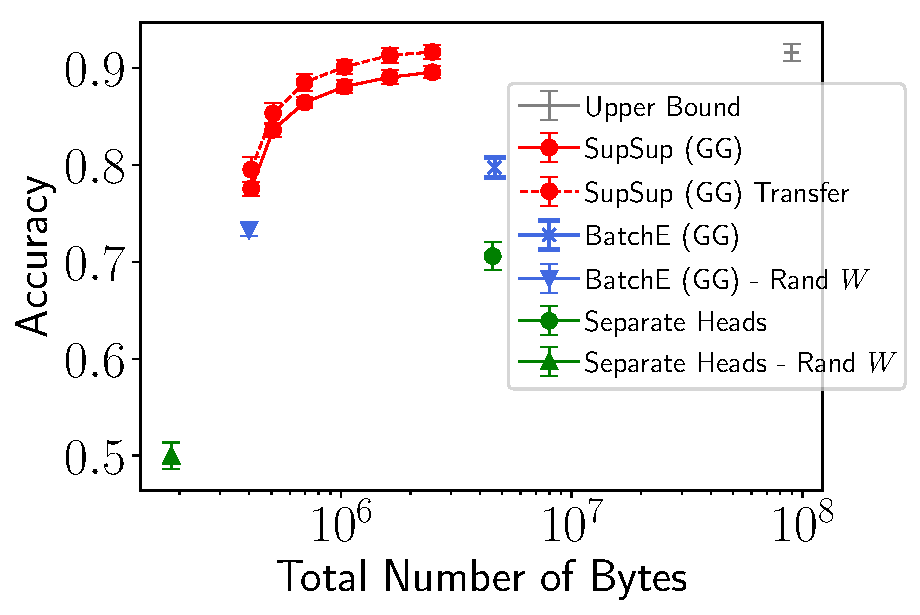
\includegraphics[width=\textwidth]{splitcifar100_full_icml.pdf}
    \label{fig:t1}
    \label{fig:splitcifar}
    \end{subfigure}
  \vspace{-1.2em}
    \caption{\textbf{(left)} \textbf{SplitImagenet} performance in Scenario \casename{GG}. \ac approaches upper bound performance with significantly fewer bytes. \textbf{(right)} \textbf{SplitCIFAR100} performance in Scenario \casename{GG} shown as mean and standard deviation over 5 seeds and splits. \ac outperforms similar size baselines and benefits from \textit{transfer}. Table in Section~\ref{sec:tables}}
    \label{fig:t1}
    \vspace{-1.2em}
\end{figure}

The correct mask $M^j$ should produce a confident, low-entropy output \cite{hendrycks2016baseline}. Therefore, to recover the correct mask we find the coefficients $\alpha$ which minimize the output entropy $\Hcal$ of $\p(\alpha)$. One option is to perform gradient descent on $\alpha$ via $\alpha \gets \alpha - \eta \nabla_\alpha \Hcal\round{\p \round{\alpha}}$
where $\eta$ is the step size, and $\alpha$s are re-normalized to sum to one after each update. Another option is to try each mask individually and pick the one with the lowest entropy output requiring $k$ forward passes. However, we want an optimization method with fixed sub-linear run time (w.r.t. the number of tasks $k$). \removed{which leads $\alpha$ to a corner of the probability simplex --- \textit{i.e.} $\alpha$ is 0 everywhere except for a single 1. We can then take the nonzero index to be the inferred task.} To this end we propose the \textit{One-Shot} and \textit{Binary} algorithms.

%\paragraph{One-Shot}
\textit{One-Shot:}
The task is inferred using a single gradient. Specifically, the inferred task is given by
    \vspace{-.2em}
\begin{equation} \label{eq:oneshot}
    \argmax_i  \round{- \frac{ \partial \Hcal\round{\p \round{\alpha}}}{\partial \alpha_i}}
    \vspace{-.6em}
\end{equation}
\removed{as entropy is decreasing maximally in this coordinate.} corresponding to one-step Frank-Wolfe algorithm~\cite{frank1956algorithm}, or one-step of gradient descent followed by softmax re-normalization with the step size approaching $\infty$.\removed{ Unless noted otherwise, $\x$ is a single image and not a batch.}
\textit{Binary:}
Resembling binary search, we infer task identity using an algorithm with $\log k$ steps. At each step we rule out half the tasks---the tasks corresponding to entries in the bottom half of $ - \nabla_\alpha \Hcal\round{\p \round{\alpha}}$. These are the coordinates in which entropy is minimally decreasing. A task $i$ is ruled out by setting $\alpha_i$ to zero and at each step we re-normalize the remaining entries in $\alpha$ so that they sum to one. \removed{Pseudo-code for both algorithms may be found in Section~\ref{sec:pseudo} of the appendix.}

Once the task is inferred the corresponding mask can be used as in Equation~\ref{eq:known-task-id} to obtain class probabilities $\p$. \removed{In both Scenario \casename{GNs} and \casename{GNu} the class probabilities $\p$ are returned.} This solution holds for \casename{GNs} and \casename{GNu}. In \casename{GNu}, $\p$ forms a distribution over the classes corresponding to the inferred task. Importantly, the superimposed forwards and backward pass (Equation~\ref{eq:sup}) is much faster than performing a separate forwards pass for each mask. \removed{, illustrated by Figure~\ref{fig:gpu_runtime}. Experiments solving thousands of tasks are detailed in \secref{exp-s23}.}
%
Because \casename{GNu} is strictly more difficult, we focus on only evaluating in Scenario \casename{GNu}. \removed{For relevant figures we provide a corresponding table in Section~\ref{sec:tables}.}


\textbf{Datasets } Experiments are conducted on PermutedMNIST, RotatedMNIST, and SplitMNIST. For PermutedMNIST \cite{kirkpatrick2017overcoming}, thousands of tasks are created each with a random permutation of MNIST pixels. For RotatedMNIST, images are rotated by 10 degrees to form 36 tasks in total (similar to \cite{cheung2019superposition}). SplitMNIST partitions MNIST into 5 different 2-way classification tasks.\removed{, each containing consecutive classes from the original dataset.}

\textbf{Training } We consider two architectures: \textbf{1)} a fully connected network with two hidden layers of size 1024 (denoted FC 1024-1024 and used in \citet{cheung2019superposition}) \textbf{2)} the LeNet 300-100 architecture \cite{lecun1989backpropagation} as used in \cite{frankle2018lottery, dettmers2019sparse}. 
For each task we train for 1000 batches of size 128 using the RMSProp optimizer \cite{tieleman2012lecture} with learning rate $0.0001$, following hyperparameters of \citet{cheung2019superposition}. Supermasks are found using the algorithm of \citet{mallya2018packnet} with threshold value 0.
\begin{figure}[t]
    \centering
            \vspace{-1em}
    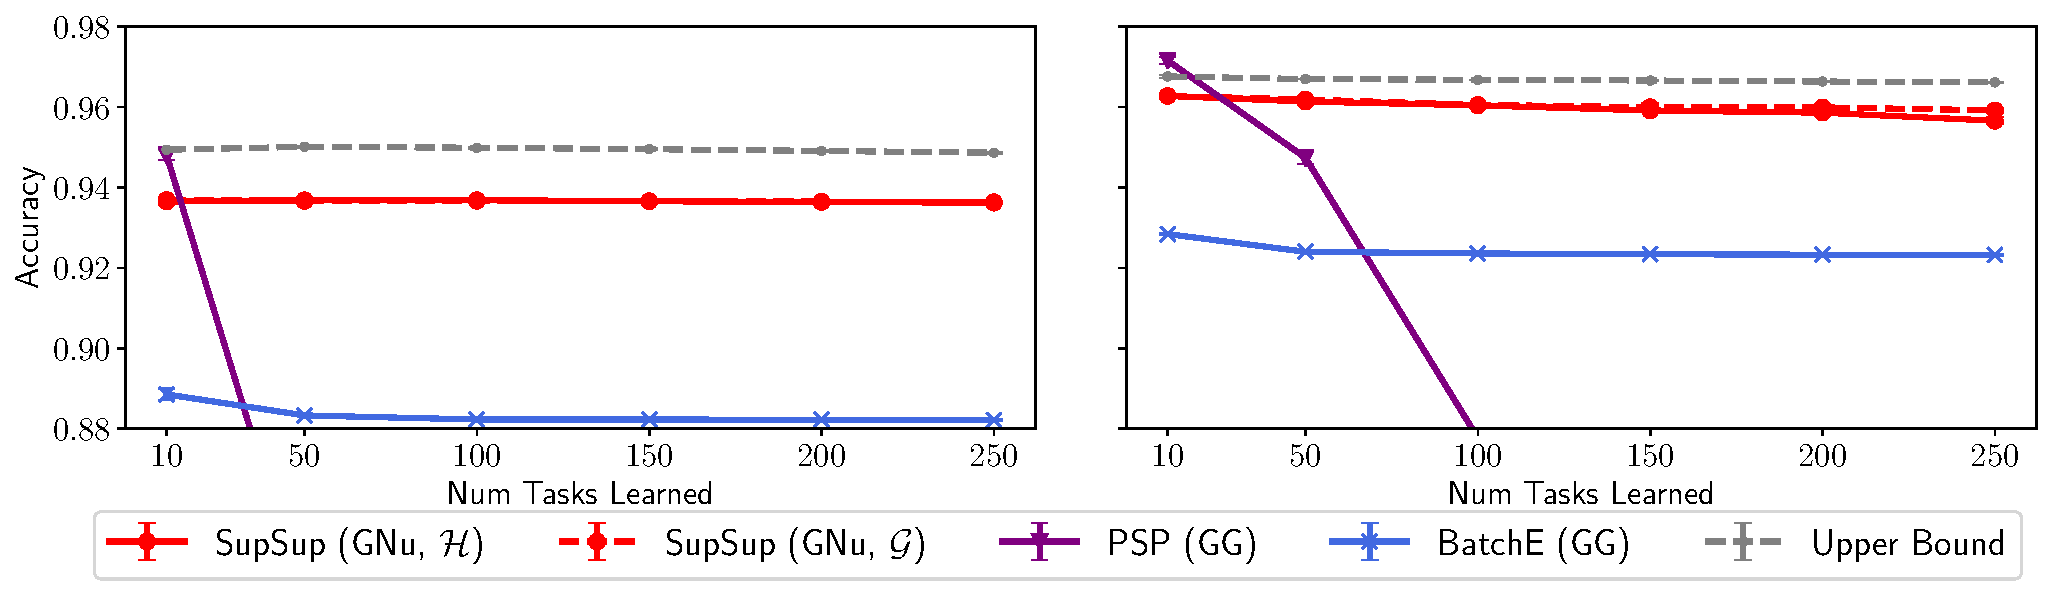
\includegraphics[width=\columnwidth]{v1-v2.pdf}
    \caption{Using \textbf{One-Shot} to infer the task, \ac outperforms methods with access to task identity. PermutedMNIST with LeNet 300-100 \textbf{(left)} and FC 1024-1024 \textbf{(right)}.}
    \vspace{-3em}
    \label{fig:v1-v2}
\end{figure}

\textbf{Evaluation } At test time we perform inference of task identity once per batch. If task is not inferred correctly then accuracy is 0 for the batch. Unless noted otherwise we showcase results for the most challenging case when the task identity inferrence uses a single image. We say ``Full Batch'' when all 128 images are used to infer task identity.

\textbf{Results } \autoref{fig:long-zoom} illustrates that \ac is able to sequentially learn 2500 permutations of MNIST. This experiment is conducted with the \textbf{One-Shot} algorithm (requiring one gradient computation) using single images to infer task identity. The same trends hold in \autoref{fig:v1-v2}, where \ac outperforms methods which operate in Scenario \casename{GG} by using the \textbf{One-Shot} algorithm to infer task identity. In \autoref{fig:v1-v2}, output sizes of 100 and 500 are respectively used for LeNet 300-100 and FC 1024-1024. The left hand side of \autoref{fig:rot-adapt} illustrates that \ac is able to infer task identity even when tasks are similar---\ac is able to distinguish between rotations of 10 degrees. Since this is a more challenging problem, we use a full batch and the \textbf{Binary} algorithm to perform task identity inference. \removed{Figure~\ref{fig:hop-infer} (appendix) shows that for HopSupSup on SplitMNIST, the new mask $\m$ converges to the correct supermask in $<30$ gradient steps.}

\textbf{Baselines \& Ablations} \autoref{fig:rot-adapt} (left) shows that even in Scenario \casename{GNu}, \ac is able to outperform PSP~\cite{cheung2019superposition} and BatchE~\cite{wen2020batchensemble} in Scenario \casename{GG}---methods using task identity. 
In \autoref{fig:rot-adapt} (right) we equip BatchE with task inference using our \textbf{One-Shot} algorithm. Instead of attaching a weight $\alpha_i$ to each supermask, we attach a weight $\alpha_i$ to each rank-one matrix \cite{wen2020batchensemble}. Moreover, in Section~\ref{sec:better-baseline} of the appendix we augment BatchE to perform task-inference using large batch sizes.
``Upper Bound'' and ``Lower Bound'' are the same as in Section~\ref{sec:S1}.

\textbf{Output Size \& an Entropy Alternative}

Empirically we find that increasing the  output size of the network significantly boosts the performance of \ac. This finding leads us to consider $\Gcal = \texttt{logsumexp}\round{\p}$ (with masked gradients for $\p_1,...,\p_\ell$) as an effective alternative to entropy. Further motivation and discussion for this objective is given in Section \ref{sec:s-neuron} of the appendix.

\begin{figure}[t]
    \centering
    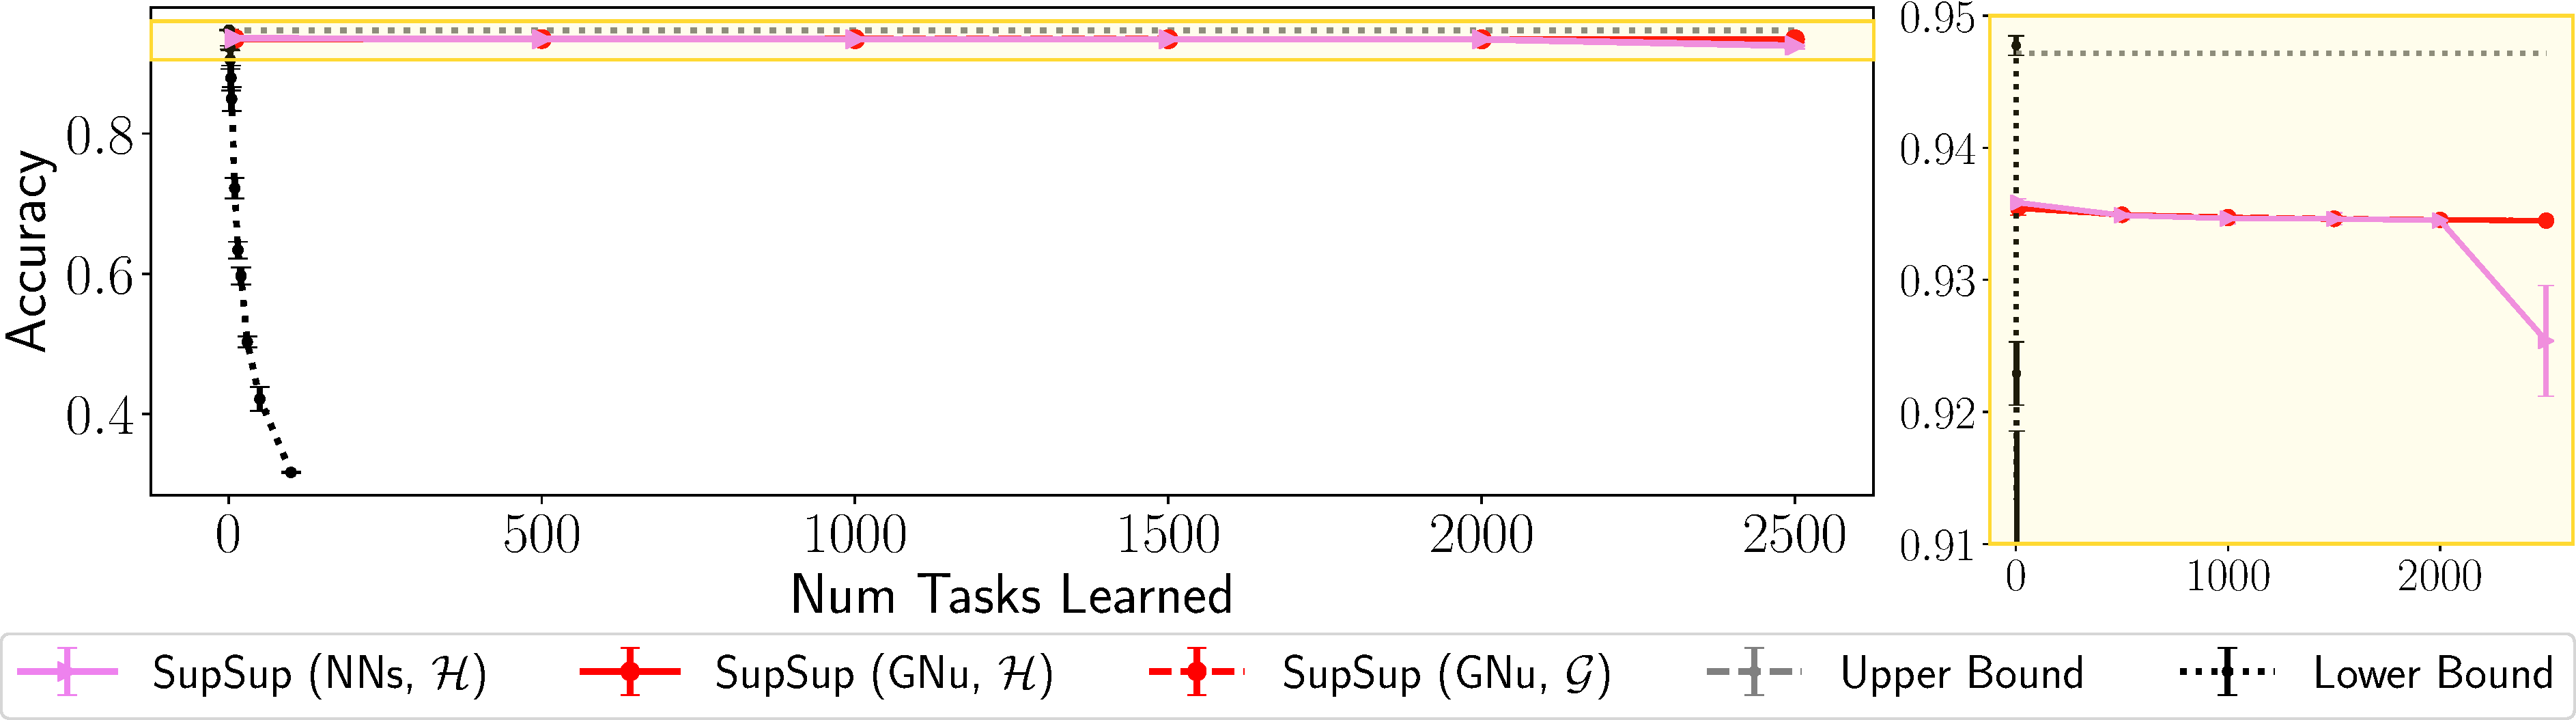
\includegraphics[width=0.5\textwidth]{long_zoom.pdf}
    \caption{Learning 2500 tasks and inferring task identity using the \textbf{One-Shot} algorithm. Results for both the \casename{GNu} and \casename{NNs} scenarios with the LeNet 300-100 model using output size 500.}
    \label{fig:long-zoom}
\end{figure}

\begin{figure}[t]
    \centering
    \vspace{-1.4em}
    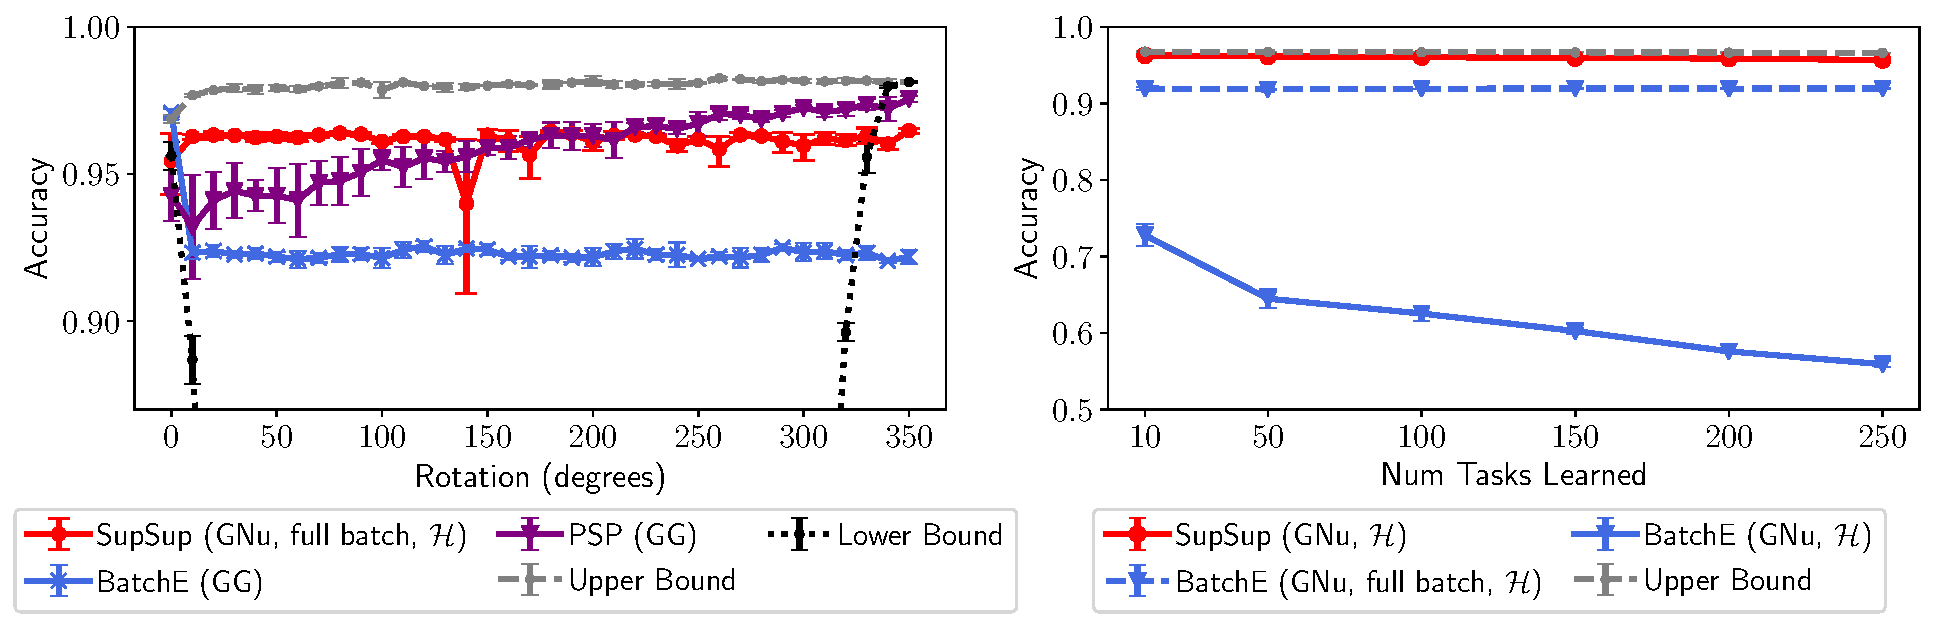
\includegraphics[width=0.5\textwidth]{rotate_adapt.pdf}
    \caption{\textbf{(left)} Testing the FC 1024-1024 model on RotatedMNIST. \ac uses \textbf{Binary} to infer task identity with a full batch as tasks are similar (differing by only 10 degrees). \textbf{(right)} The \textbf{One-Shot} algorithm can be used to infer task identity for BatchE \cite{wen2020batchensemble}. Experiment conducted with FC 1024-1024 on PermutedMNIST using an output size of 500, shown as mean and stddev over 3 runs.}
    \label{fig:rot-adapt}
    \vspace{-1.5em}
\end{figure}

\subsection{Scenario \casename{NNs}: No Task Identity During Training or Inference} \label{sec:S4}
Automatic task inference enables the further extension of \ac to Scenario \casename{NNs}, where task identity is entirely unknown (even during training). 
A new supermask is allocated whenever \ac is uncertain about the current task identity, and $k$ (the number of tasks learned so far) is incremented.

We consider the \textbf{One-Shot} algorithm and say that \ac is uncertain when performing task identity inference if $\nu = \texttt{softmax}\round{-\nabla_\alpha \Hcal \round{\p\round{\alpha}}}$ is approximately uniform. Specifically, if $k \max_i \nu_i < 1 + \epsilon $ a new mask is allocated and $k$ is incremented. Otherwise mask $\argmax_i \nu_i$ is used, which corresponds to Equation~\ref{eq:oneshot}. We consider PermutedMNIST and conduct experiments on learning up to 2500 tasks entirely without any task information. \autoref{fig:long-zoom} shows that \ac in Scenario \casename{NNs} achieves comparable performance even to Scenario \casename{GNu}, entirely removing the need of knowing task identity.
We train on each task for 1000 iteraions (iteration number unknown to the model). Every 100 batches the model must choose to allocate a new mask or pick an existing mask using the above criteria ($\epsilon = 2^{-3}$). 
\vspace*{-1ex}
\section{Conclusion}
\vspace*{-1ex}
Supermasks in Superposition (\ac) is a flexible and compelling model applicable to a wide range of scenarios in continual learning. \ac leverages the power of subnetworks\removed{~\cite{zhou2019deconstructing, ramanujan2019s, mallya2018packnet}}, and gradient-based optimization to infer task identity when unknown. 
\ac achieves state-of-the-art performance on SplitImageNet when given task identity, and scales to thousands of permutations and almost indiscernible rotations of MNIST without any task information. 

\removed{A limitation we observed has to do with task identity inference when models are not well calibrated---models that are overly confident for the wrong task. As future work, we hope to explore
automatic task inference with more calibrated models~\cite{guo2017calibration}, as well as circumventing calibration challenges by using  optimization objectives such as self-supervision \cite{he2019momentum} and energy based models \cite{grathwohl2019your}. In doing so, we hope to tackle large-scale problems in Scenarios \casename{GN} and \casename{NNs}.}

{
\bibliographystyle{icml2020}
\bibliography{ref}
}

\clearpage

\appendix

\setcounter{figure}{7} 
\section{Algorithm pseudo-code} \label{sec:pseudo}
Algorithms \ref{alg:oneshot} and \ref{alg:binary} respectively provide pseudo-code for the \textbf{One-Shot} and \textbf{Binary} algorithms detailed in Section~\ref{sec:S23}. Both aim to infer the task $j \in \{1,...,k\}$ associated with input data $\x$.

\begin{algorithm}[tb]
\caption{One-Shot$(f, \x, W, k, \{M^i\}_{i=1}^k, \Hcal)$} \label{alg:oneshot}
\begin{algorithmic}[1]
\STATE{$\alpha \gets \begin{bmatrix} \frac{1}{k} & \frac{1}{k} &... &\frac{1}{k}  \end{bmatrix}$} 
\STATE{$\p \gets f\round{\x, W \odot \round{ \sum_{i=1}^k \alpha_i M^i}} $} 
\STATE{$\textbf{return} \ \argmax_i  \round{- \frac{ \partial \Hcal\round{\p}}{\partial \alpha_i}}$}
\end{algorithmic}
\end{algorithm}

\begin{algorithm}[tb]
\caption{Binary$(f, \x, W, k, \{M^i\}_{i=1}^k, \Hcal)$}\label{alg:binary}
\begin{algorithmic}[1] 
\STATE{$\alpha \gets \begin{bmatrix} \frac{1}{k} & \frac{1}{k} &... &\frac{1}{k}  \end{bmatrix}$} 
\WHILE{$\norm{0}{\alpha} > 1$} 
    \STATE{$\p \gets f\round{\x, W \odot \round{ \sum_{i=1}^k \alpha_i M^i}} $} 
    \STATE{$g \gets - \nabla_\alpha \Hcal\round{\p}$} 
    \FOR{$i \in \{1,...,k\}$} 
        \IF{$g_i \leq \textbf{median}\round{g}$}
            \STATE{$\alpha_i \gets 0$} 
        \ENDIF
    \ENDFOR
    \STATE{$\alpha \gets \alpha /\norm{1}{\alpha} $} 
\ENDWHILE
\STATE{$\textbf{return} \ \argmax_i  \alpha_i$}
\end{algorithmic}
\end{algorithm}

\section{Extended Related Work} \label{sec:ext-rw}


\textbf{Regularization based methods }
Methods like Elastic Weight Consolidation (EWC) \cite{kirkpatrick2017overcoming} and Synaptic Intelligence (SI) \cite{zenke2017continual} penalize the movement of parameters that are important for solving previous tasks 
in order to mitigate catastrophic forgetting.
\removed{Measures of parameter importance vary; e.g. EWC uses the Fisher Information matrix \cite{pascanu2013revisiting}.} These methods operate in the \casename{GNs} scenario (\tabref{scenarios}).
They ameliorate but do not exactly eliminate catastrophic forgetting.

%\vivekr{Given that there is no structural change to the network in these methods, they will still encounter some forgetting when attempting to learn a large number of tasks.}
%\rosanne{Nice! How about "encounter forgetting and/or suffer in new task performances" when k is large?}

%\paragraph{(2) Using Exemplars, Replay, or Generative models}
\textbf{Using exemplars, replay, or generative models }
These methods explicitly (\cite{rebuffi2017icarl, lopez2017gradient, chaudhry2018efficient} or implicitly (with generative models, \cite{rolnick2019experience, shin2017continual}) capture data from previous tasks. 
Exact replay of the entire dataset can prevent catastrophic forgetting but at great time and memory cost. Generators in generative approaches are still susceptible to forgetting.

\section{Output Size and an Alternative Metric} \label{sec:s-neuron}
In contrast with previous methods, \ac is performing $\ell k$-way classification without $\ell k$ output neurons. Given data during inference \textbf{1)} the task is inferred and \textbf{2)} the corresponding mask is used to obtain outputs $\p$. The class probabilities $\p$ correspond to the classes for the inferred task, effectively reusing the neurons in the final layer. 

\ac could use an output size of $\ell$, though we find in practice that it helps significantly to add extra neurons to the final layer (Figure~\ref{fig:v1-v2-sz}). Specifically we consider outputs $\p \in \R^{s}$ and refer to the neurons $\{\ell+1,...,s\}$ as superfluous neurons (s-neurons). The standard cross-entropy loss will push the values of s-neurons down throughout training. Accordingly, we consider an objective $\Gcal$ which encourages the s-neurons to have large negative values and can be used as an alternative to entropy in Equation~\ref{eq:oneshot}. Given data from task $j$, mask $M^j$ will minimize the values of the s-neurons as it was trained to do. Other masks were also trained to minimize the values of the s-neurons, but not for data from task $j$. Therefore we consider $ \Gcal = \texttt{logsumexp}\round{\p}$ (with masked gradients for $\p_1,...,\p_\ell$) as an effective alternative to entropy.

\begin{figure}[t]
    \centering
    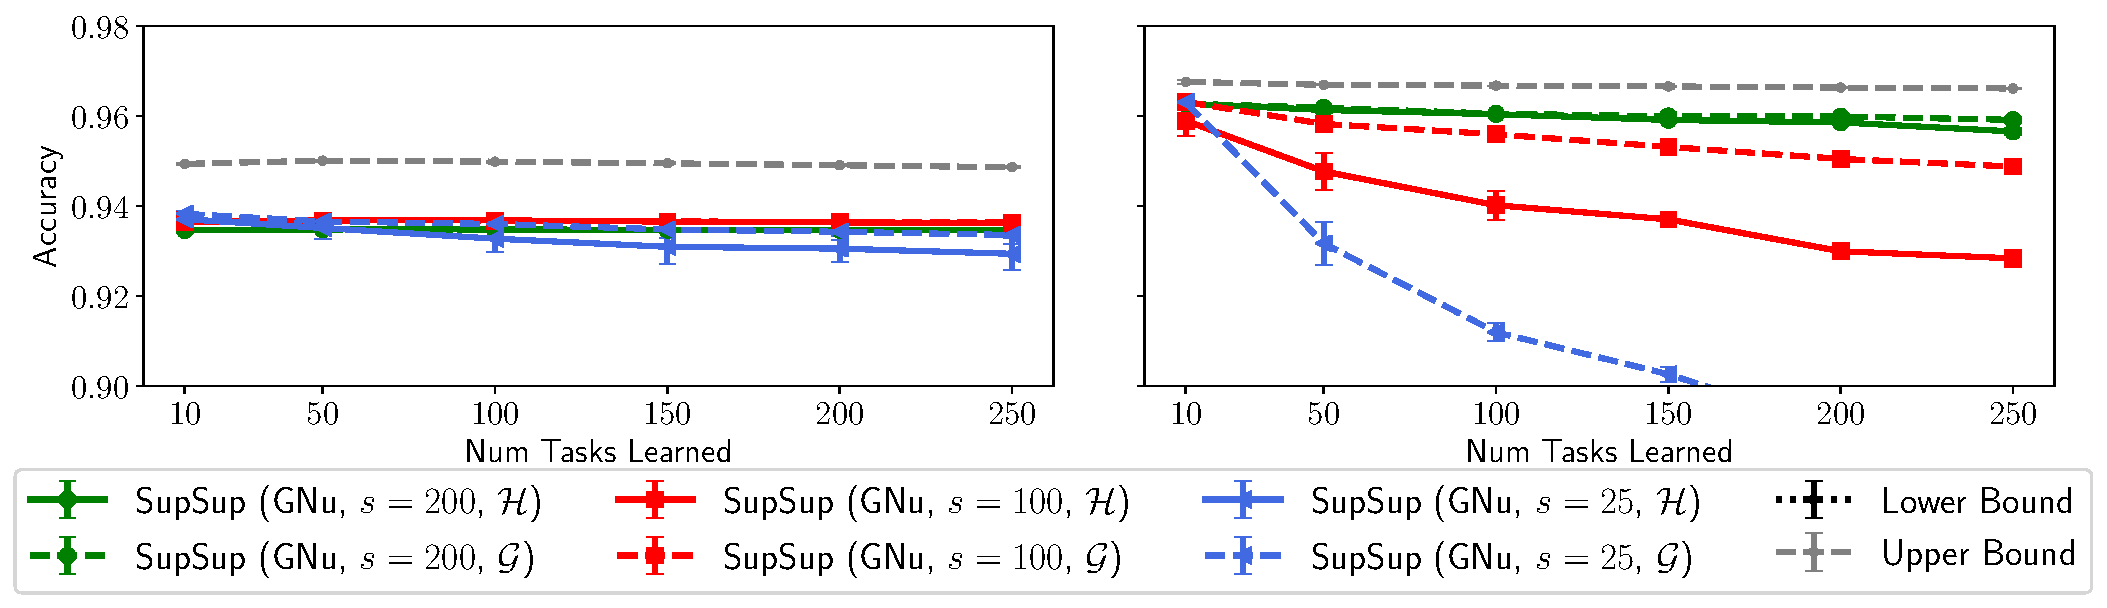
\includegraphics[width=0.5\textwidth]{v1-v2-sz.pdf}
    \caption{The effect of output size $s$ on \ac using the \textit{One-Shot} algorithm. Results shown for PermutedMNIST with LeNet 300-100 \textbf{(left)} and FC 1024-1024 \textbf{(right)}.}
    \label{fig:v1-v2-sz}
    \vspace{-1em}
\end{figure}


\section{Augmenting BatchE For Scnario \casename{GNu}} \label{sec:better-baseline}

In Section~\ref{sec:S23} we demonstrate that BatchE \cite{wen2020batchensemble} is able to infer task identity using the \textbf{One-Shot} algorithm. In this section we show that, equipped with $\Hcal$ from Section~\ref{sec:method}, BatchE can also infer task identity by using a large batch size. We refer to this method as Augmented BatchE (ABatchE).

For clarity we describe ABatchE for one linear layer, \textit{i.e.} we describe the application of ABatchE to
\begin{align}
    f(\x, W) = \texttt{softmax}\round{W^\top \x}
\end{align}
for input data $\x \in \R^m$ and weights  $W \in \R^{m \times n}$. In BatchE \cite{wen2020batchensemble}, $W$ is trained on the first task then frozen. For task $i$ BatchE learns ``fast weights'' $r_i \in \R^{m}$, $s_i \in \R^{n}$ and outputs are computed via
\begin{align} \label{eq:ogbe}
    f(\x, W) = \texttt{softmax}\round{\round{W \odot r_i s_i^\top  }^\top \x}.
\end{align}
\citet{wen2020batchensemble} further demonstrate that Equation~\ref{eq:ogbe} can be vectorized as
\begin{align} \label{eq:vbe}
    f(\x, W) = \texttt{softmax}\round{ \round{W^\top \round{\x \odot r_i }} \odot s_i }
\end{align}
or, for a batch of data $X \in \R^{b \times m}$,
\begin{align} \label{eq:bvbe}
    f(X, W) = \texttt{softmax}\round{ \round{\round{X \odot R^{b}_i }  W} \odot S^{b}_i }.
\end{align}
In Equation~\ref{eq:bvbe}, $R^b_i \in \R^{b \times m}$ is a matrix where each of the $b$ rows is $r_i$ (likewise $S^b_i \in \R^{b \times n}$ is a matrix where each of the $b$ rows is $s_i$).
\begin{figure*}[t]
    \centering
    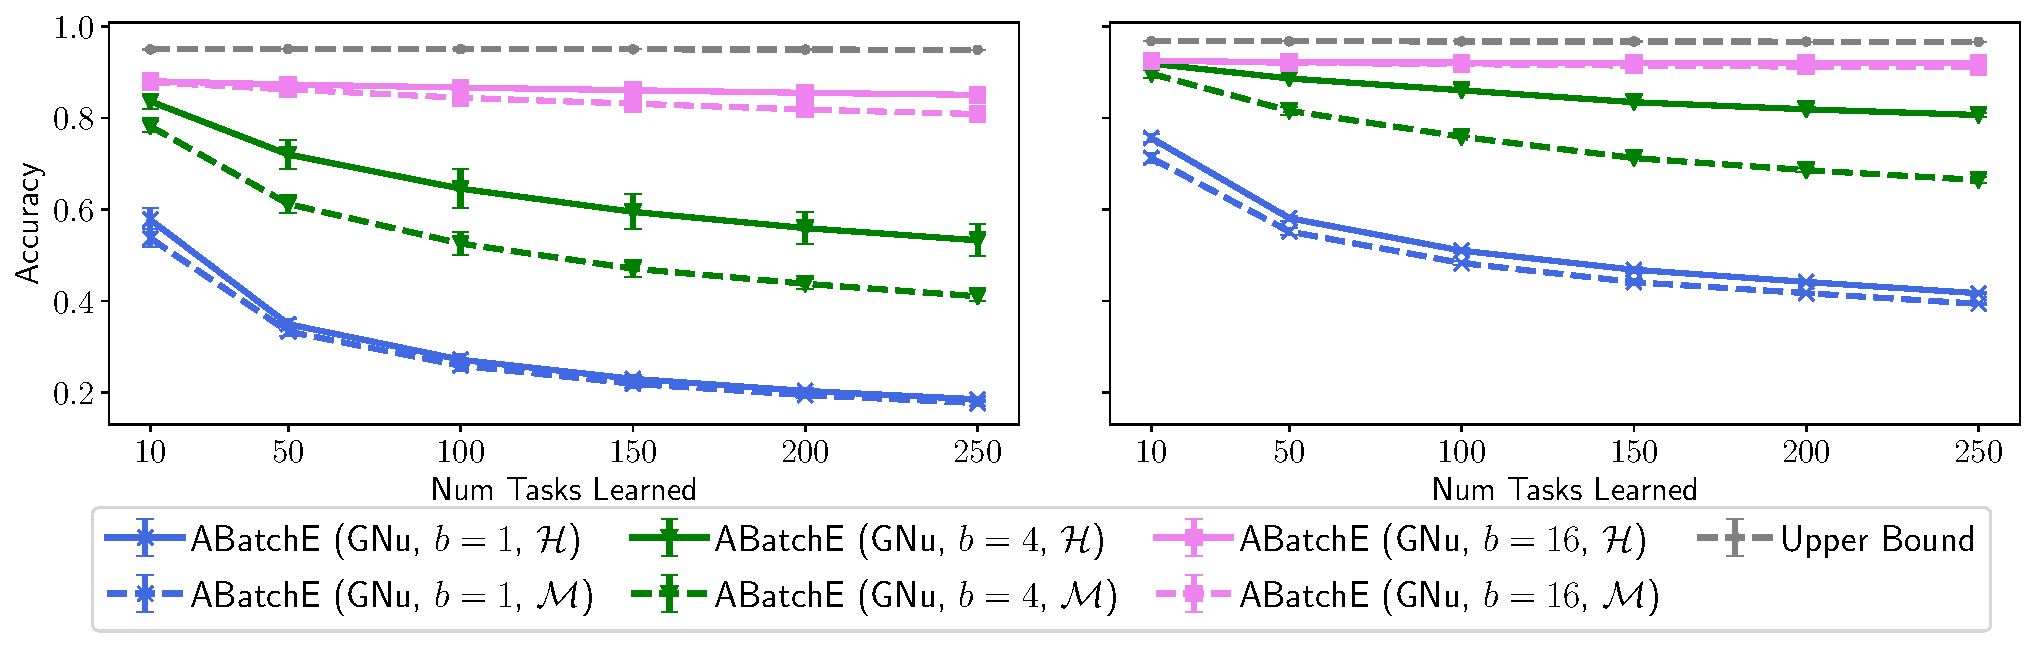
\includegraphics[width=\textwidth]{figs/abe.pdf}
    \caption{Testing ABatchE on PermutedMNIST with LeNet 300-100 \textbf{(left)} and FC 1024-1024 \textbf{(right)} with output size 100.}
    \label{fig:abe}
    \vspace{-1.5em}
\end{figure*}
As in Section~\ref{sec:S23} we now consider the case where data $X \in \R^{b \times m}$ comes from task $j$ but this information is not known to the model. For ABatchE we repeat the data $k$ times, where $k$ is the number of tasks learned so far, and use different ``fast weights'' for each repetiton. Specifically, we consider repeated data $\tilde X \in \R^{bk \times m}$ and augmented matricies $\tilde R \in \R^{bk \times m}$ and $\tilde S \in \R^{bk \times n}$ given by
\begin{align}
\tilde X = \begin{bmatrix} X \\ X \\ \vdots \\ X \end{bmatrix}, \ \ \ \ \ \tilde R =\begin{bmatrix} R^b_1 \\ R^b_2 \\ \vdots \\ R^b_k \end{bmatrix},  \ \ \ \ \   \tilde S =\begin{bmatrix} S^b_1 \\ S^b_2 \\ \vdots \\ S^b_k \end{bmatrix} .
\end{align}
Outputs are then computed as
\begin{align} \label{eq:bvabe}
    f(X, W) = \texttt{softmax}\round{ \round{\round{\tilde X \odot \tilde R }  W} \odot \tilde S }
\end{align}
where the $b$ rows $(bi,...,bi + b-1)$ of the output correspond exactly to Equation~\ref{eq:bvbe}. The task may then be inferred by choosing the $i$ for which the rows $(bi,...,b(i+1) - 1)$ minimize the objective $\Hcal$. If $f(X, W)_i$ denotes row $i$ of $f(X, W)$ then for objective $\Hcal$ the inferred task for ABatchE is
\begin{align}
    \argmin_i \sum_{\omega = 0}^{b-1} \Hcal\round{f(X, W)_{bi + \omega}}.
\end{align}
To extend ABatchE to deep neural networks the matricies $\tilde R$ and $\tilde S$ are constructed for each layer.

One advantage of ABatchE over \ac is that no backwards pass is required. However, ABatchE uses a very large batch size for large $k$, and the forward pass therefore requires more compute and memory. %\vivekr{and memory}\vivekr{end this sentence here} as it includes more matrix multiplication. 
Another disadvantage of ABatchE is that the performance of ABatchE is limited by the performance of BatchE. In Section~\ref{sec:S23} we demonstrate that \ac outperforms BatchE when BatchE is given task identity information.

Since the objective for ABatchE need not be differentiable we also experiment with an alternative metric of confidence $\Mcal(\p) = -\max_i \p_i$.
We showcase results for ABatchE on PermutedMNIST in \autoref{fig:abe} for various values of $b$. The entropy objective $\Hcal$ performs better than $\Mcal$, and forgetting is only mitigated when using 16 images ($b=16$). With 250 tasks, $b=16$ corresponds to a batch size of 4000.

\section{Extended Training Details} \label{sec:hyperparams}
\subsection{SplitCIFAR-100 (\casename{GG})}

As in \cite{wen2020batchensemble} we train each model for 250 epochs per task. We use standard hyperparameters---the Adam optimizer \cite{kingma2014adam} with a batch size of 128 and learning rate 0.001 (no warmup, cosine decay \cite{cosine}). For \ac we follow \cite{ramanujan2019s} and use non-affine normalization so there are no learned parameters. We found it better to use a higher learning rate (0.1) when training BatchE (Rand $W$), and the BatchE number is taken from \cite{wen2020batchensemble}. Instead of training separate heads per tasks when training BatchE (Rand $W$), we apply the rank one pertubation to the final layer.

\section{Corresponding Tables}\label{sec:tables}
In this section we provide tabular results corresponding to \autoref{fig:t1} \textbf{(right)}.
\begin{table}[H]
    \centering
    \caption{Accuracy on SplitCIFAR100 corresponding to \autoref{fig:t1} \textbf{(right)}. \ac with Transfer approaches upper bound.}
    \begin{tabular}{llr}
\toprule
                                          Entry &         Avg Acc@1 &    Bytes \\
\midrule
SupSup ($\ensuremath{\mathsf{GG}}$) &  $77.56~\pm 0.73$ &    408432 \\
SupSup ($\ensuremath{\mathsf{GG}}$) &  $83.62~\pm 0.74$ &    508432 \\
SupSup ($\ensuremath{\mathsf{GG}}$) &  $86.45~\pm 0.61$ &    695592 \\
SupSup ($\ensuremath{\mathsf{GG}}$) &  $88.09~\pm 0.64$ &   1035792 \\
SupSup ($\ensuremath{\mathsf{GG}}$) &  $89.06~\pm 0.75$ &   1630032 \\
SupSup ($\ensuremath{\mathsf{GG}}$) &  $89.57~\pm 0.64$ &   2487472 \\
SupSup ($\ensuremath{\mathsf{GG}}$) Transfer &  $79.53~\pm 1.31$ &    408432 \\
SupSup ($\ensuremath{\mathsf{GG}}$) Transfer &  $85.33~\pm 1.05$ &    508432 \\
SupSup ($\ensuremath{\mathsf{GG}}$) Transfer &  $88.52~\pm 0.85$ &    695592 \\
SupSup ($\ensuremath{\mathsf{GG}}$) Transfer &  $90.12~\pm 0.75$ &   1035792 \\
SupSup ($\ensuremath{\mathsf{GG}}$) Transfer &  $91.31~\pm 0.74$ &   1630032 \\
SupSup ($\ensuremath{\mathsf{GG}}$) Transfer &  \textbf{91.66} $~\pm 0.74$ &   2487472 \\
BatchE ($\ensuremath{\mathsf{GG}}$) &  $79.75~\pm 1.00$ &   4640800 \\
BatchE ($\ensuremath{\mathsf{GG}}$) - Rand $W$ &  $74.96~\pm 0.68$ &    400240 \\
Separate Heads &  $70.60~\pm 1.40$ &   4544560 \\
Separate Heads - Rand $W$ &  $50.00~\pm 1.37$ &    184000 \\\midrule
Upper Bound &  $91.62~\pm 0.89$ &  89675200 \\
\bottomrule
\end{tabular}


    \label{tab:t1}
\end{table}

\subsection{SplitImageNet (\casename{GG})}
We use the Upper Bound and BatchE number from \cite{wen2020batchensemble}. For \ac we train for 100 epochs with a batch size of 256 using the Adam optimizer \cite{kingma2014adam} with learning rate 0.001 (5 epochs warmup, cosine decay \cite{cosine}).

\subsection{\casename{GNu} Experiments}
We clarify some experimental details for \casename{GNu} experiments \& baselines. For the BatchE \cite{wen2020batchensemble} baseline we find it best to use kaiming normal initialization with a learning rate of 0.01 (0.0001 for the first task when the weights are trained). As we are considering hundreds of tasks, instead of training separate heads per tasks when training BatchE we also apply the rank one pertubation to the final layer. PSP \cite{cheung2019superposition} provides MNISTPerm results so we use the same hyperparameters as in their code. We compare with rotational superposition, the best performing model from PSP.

\subsection{Speed of the Masked Forward Pass}

We now provide justification for the calculation mentioned in Section~\ref{sec:S1}---when implemented properly the masking operation should require $\sim 1\%$ of the total time for a forward pass (for a ResNet-50 on a NVIDIA GTX 1080 Ti GPU). It is reasonable to assume that selecting indices is roughly as quick as memory access. A NVIDIA GTX 1080 Ti has a memory bandwidth of 480 GB/s. A ResNet-50 has around $2.5\cdot 10^7$ 4-byte (32-bit) parameters---roughly 0.1 GB. Therefore, indexing over a ResNet-50 requires at most $0.1 \text{ GB} / \left(480\text{ GB/s}\right) \approx 0.21\text{ ms}$. For comparison, the average forward pass of a ResNet-50 for a $3\times 224\times 224$ image on the same GPU is about 25 ms. 

Note that NVIDIA hardware specifications generally assume best-case performance with sequential page reads. However, even if real-world memory bandwidth speeds are 60-70\% slower than advertised, the fraction of masking time would remain in the $\leq 3$\% range.

\end{document}
